% Created 2016-03-18 Fri 15:53
\documentclass[a4paper,12pt]{article}
\usepackage[utf8x]{inputenc}
\usepackage[T1]{fontenc}
\usepackage{fixltx2e}
\usepackage{graphicx}
\usepackage{longtable}
\usepackage{float}
\usepackage{wrapfig}
\usepackage{rotating}
\usepackage[normalem]{ulem}
\usepackage{amsmath}
\usepackage{textcomp}
\usepackage{marvosym}
\usepackage{wasysym}
\usepackage{amssymb}
\usepackage{hyperref}
\tolerance=1000
\usepackage{fancyvrb}
\setlength{\textheight}{24cm}
\setlength{\textwidth}{16cm}
\setlength{\evensidemargin}{-0cm}
\setlength{\oddsidemargin}{-0cm}
\setlength{\topmargin}{0cm}
\renewcommand{\baselinestretch}{1.1}%1.1
\author{Hans Fangohr}
\date{\today}
\title{Class diagrams}
\hypersetup{
  pdfkeywords={},
  pdfsubject={},
  pdfcreator={Emacs 24.5.1 (Org mode 8.2.10)}}
\begin{document}

\maketitle
\tableofcontents



\section{OOMMF Classes}
\label{sec-1}


Inheritance structure taken from \url{http://math.nist.gov/oommf/doc/userguide12a6/userguide/Standard_Oxs_Ext_Child_Clas.html#BA}, with additional reading of source code in \verb~oommf/app/oxs/base~ and \verb~oommf/app/oxs/ext~

\subsection{Atlasses}
\label{sec-1-1}

Figure \ref{fig:atlas} on page \pageref{fig:atlas} shows the OOMMF Atlas classes.

\begin{figure}[htb]
\centering
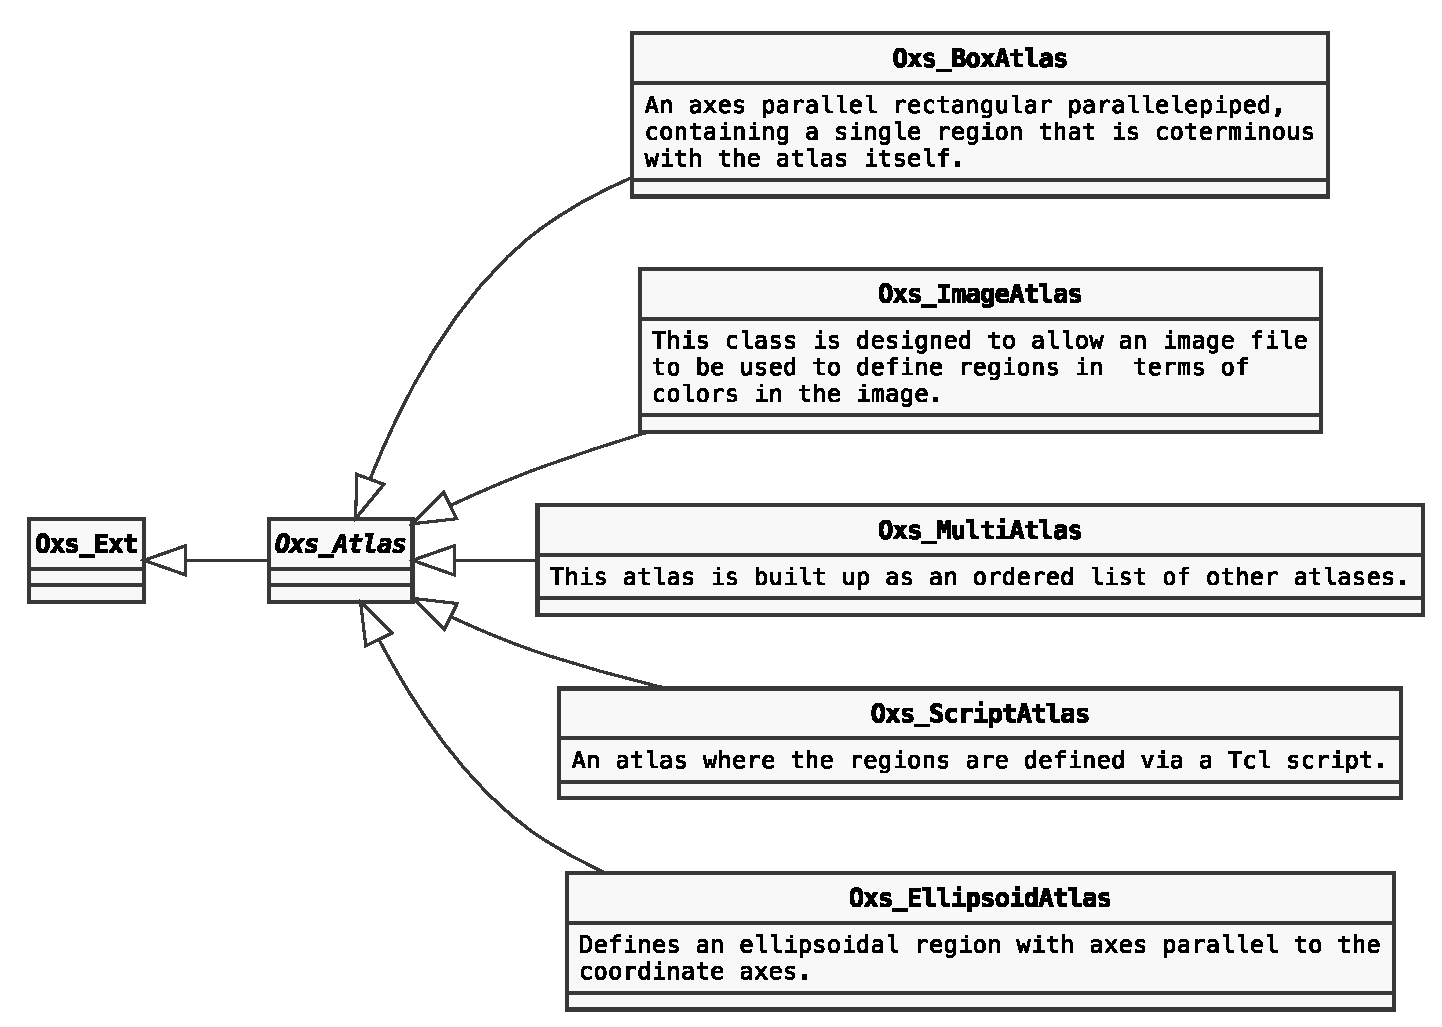
\includegraphics[width=1\textwidth]{atlas.eps}
\caption{\label{fig:atlas}OOMMF Atlas classes}
\end{figure}

\subsection{Meshes}
\label{sec-1-2}

Figure \ref{fig:mesh} on page \pageref{fig:mesh} shows the OOMMF Mesh classes.

\begin{figure}[htb]
\centering
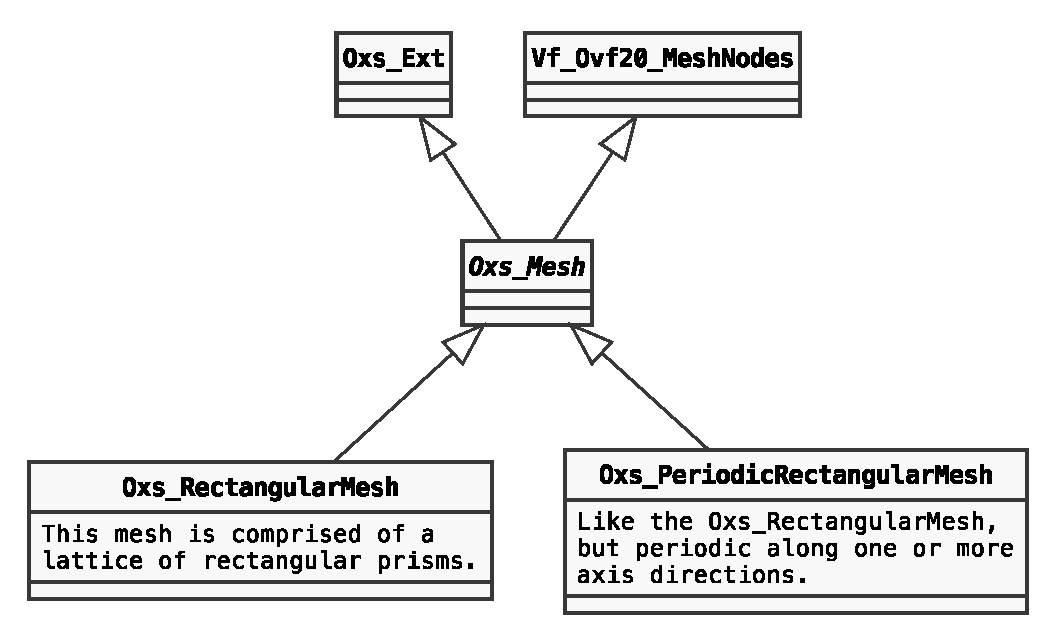
\includegraphics[width=1\textwidth]{mesh.eps}
\caption{\label{fig:mesh}Mesh classes}
\end{figure}

\subsection{Energies}
\label{sec-1-3}
\subsubsection{Anisotropy energy}
\label{sec-1-3-1}

Figure \ref{fig:anisotropy-energy} on page \pageref{fig:anisotropy-energy} shows the OOMMF anisotropy energy classes.

\begin{figure}[htb]
\centering
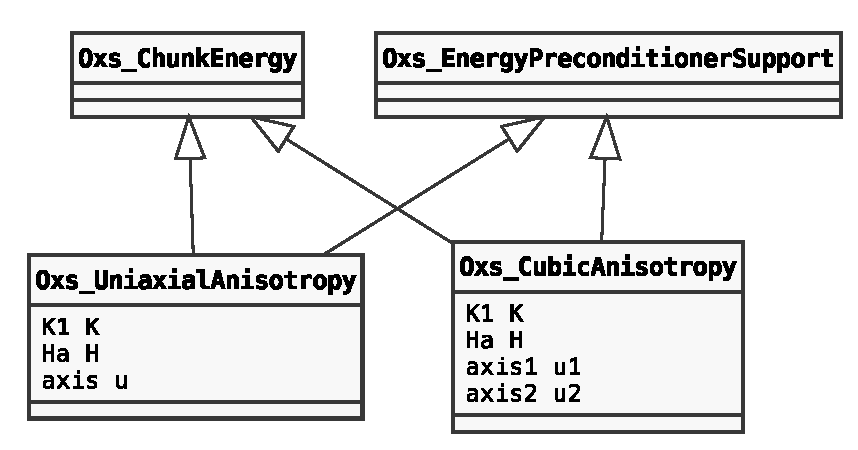
\includegraphics[width=1\textwidth]{anisotropy-energy.eps}
\caption{\label{fig:anisotropy-energy}Anisotropy energy classes}
\end{figure}


\#+LATEX \clearpage\newpage

\section{Setting up your system to compile this file}
\label{sec-2}

\subsection{Mini tutorial generating UML diagrams}
\label{sec-2-1}

\begin{itemize}
\item Install 'plantuml' on your system
\begin{itemize}
\item \verb~brew install plantuml~ on OS X
\end{itemize}
\item Tell Emacs where to find the plantuml jar file (in \textasciitilde{}.emacs):
\begin{Verbatim}
(setq org-plantuml-jar-path~
    (expand-file-name "/usr/local/Cellar/plantuml/8031/plantuml.8031.jar"))
\end{Verbatim}

\item Tell Emacs to parse plantuml code (also python, sh, dot in this example):

\begin{Verbatim}
;; enable python for in-buffer evaluation
(org-babel-do-load-languages
 'org-babel-load-languages
 '(
   (python . t)
   (sh . t)
   (plantuml . t)
   (dot . t)
   ))

;; all plantuml and dot code to execute without confirmation
(defun my-org-confirm-babel-evaluate (lang body)
(not (or (string= lang "plantuml") (string= lang "dot"))))
(setq org-confirm-babel-evaluate 'my-org-confirm-babel-evaluate)
\end{Verbatim}

\item To re-execute the plantuml code, use \verb~C-c C-c~ when the cursor is in that block.

\item Let's add \verb~*.eps~ files to the repository, so that we only need this
setup for creating new class diagrams.
\end{itemize}

\subsection{To compile the pdf from this file (watch how the screen changes):}
\label{sec-2-2}
\verb~C-c C-e l p~
% Emacs 24.5.1 (Org mode 8.2.10)
\end{document}
